
\subsection*{5.1 Data Representation}
Data representation is crucial in statistics for organizing and analyzing information. Various methods are used to display and interpret data effectively.

\textbf{Key Concepts:}

\begin{itemize}
	\item \textbf{Tables:} Data can be organized in tables for better readability and analysis.
	\item \textbf{Bar Charts:} Used to represent categorical data with rectangular bars. Horizontal axis of a bar chart can be numberical or descriptive.
	\item \textbf{Pie Charts:} Circular charts divided into sectors, where each sector represents a proportion of the whole.
	\item \textbf{Histograms:} Graphical representation of grouped data with bars whose areas represent frequency. Although visually similar to bar charts histograms visualize quantitative data or numerical data, whereas bar charts display categorical variables. Veritably axis of histogram represent frequency while horizontal some numerical data. (see Example 2).
	\item \textbf{Frequency Distributions:} Tables that display the frequency of different outcomes in a dataset.
	\item \textbf{Cumulative Frequency Tables:} Tables that show the accumulation of frequencies up to a given class interval.
	\item \textbf{Cumulative Frequency Curve (Ogive):} A graphical representation of cumulative frequency that helps estimate median, percentiles, and quartiles.
	
\end{itemize}

\textbf{Examples:}

\begin{flushleft}
	\textbf{Example 1: Construct a frequency distribution table from the given data:} \\
	\{3, 5, 7, 3, 5, 7, 9, 7, 5, 3, 7, 5, 9, 7, 5\}
	
	\vspace{0.5cm}
	\textbf{Solution:}
	\vspace{0.5cm}
	
	\begin{center}
		\begin{tabular}{c|c}
			\textbf{Value (x)} & \textbf{Frequency (f)} \\
			\hline
			3 & 3 \\
			5 & 4 \\
			7 & 5 \\
			9 & 2 \\
		\end{tabular}
	\end{center}
	
	The frequency table summarizes the given dataset.
\end{flushleft}

\begin{flushleft}
	\textbf{Example 2: The table below shows the marks obtained by students in a test. Construct a histogram.}
	
	\vspace{0.5cm}
	
	\begin{center}
		\begin{tabular}{c|c}
			\textbf{Marks Range} & \textbf{Frequency} \\
			\hline
			0-10 & 2 \\
			10-20 & 4 \\
			20-30 & 7 \\
			30-40 & 10 \\
			40-50 & 6 \\
		\end{tabular}
	\end{center}
	
	\vspace{0.5cm}
	\textbf{Solution:}
	\vspace{0.5cm}
	
	A histogram is a bar graph where the class intervals are plotted on the x-axis, and the frequencies are represented by the heights of the bars.
	\begin{center}
		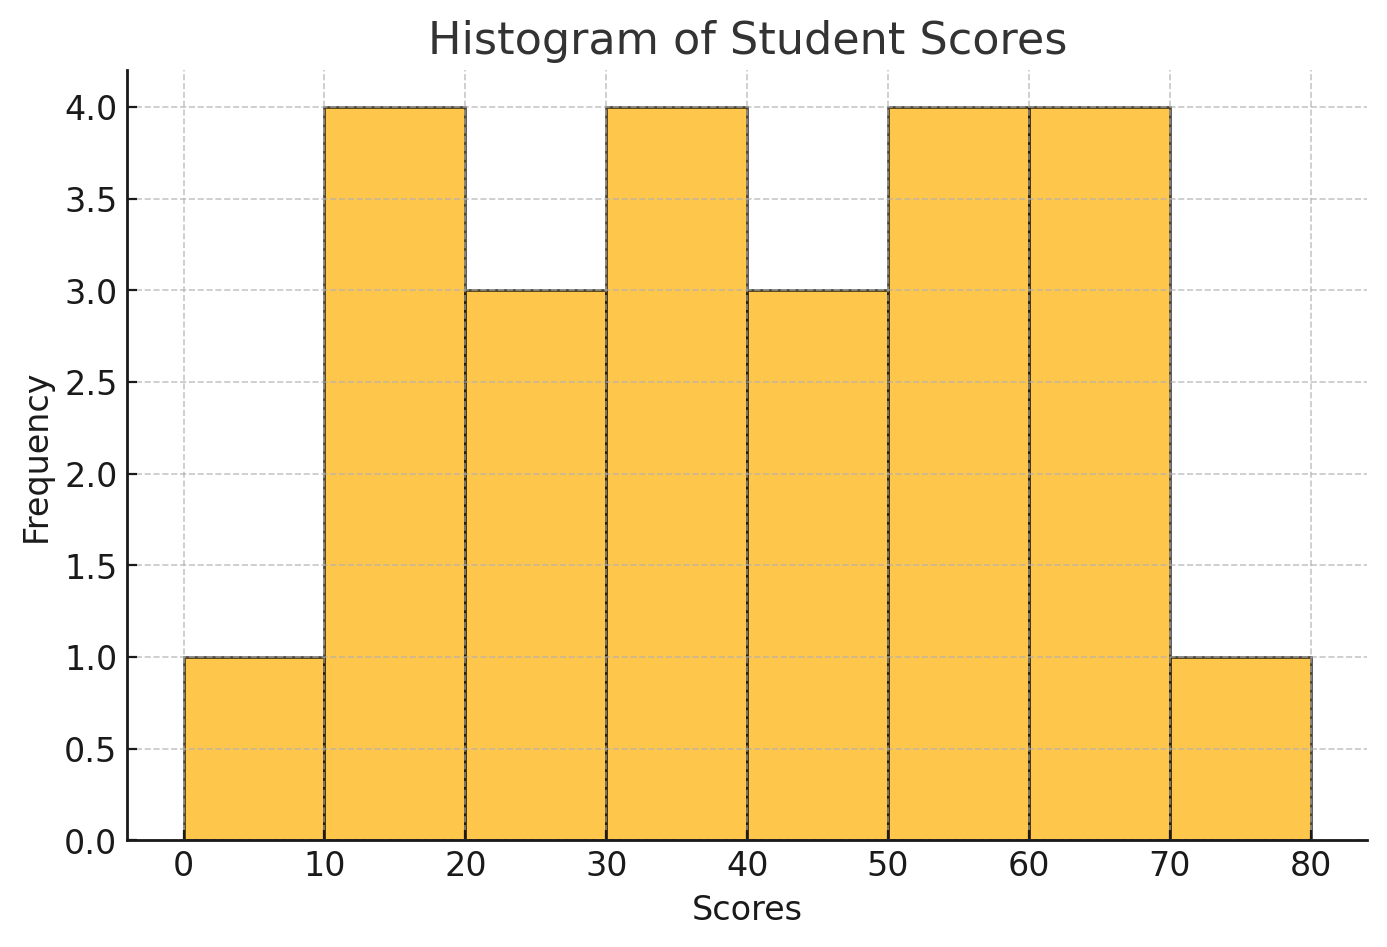
\includegraphics[width=0.6\textwidth]{5.1.png}
		\captionof{figure}{Histogram of student marks.}
	\end{center}
	Note that vertical axis represent frequency (always) while horizontal axis represents some numerical data (in this case students score).
\end{flushleft}

\begin{flushleft}
	\textbf{Example 3: The pie chart below represents the distribution of students in a school. If the total number of students is 600, find the number of students in each category.}
	
	\vspace{0.5cm}
	
	\begin{center}
		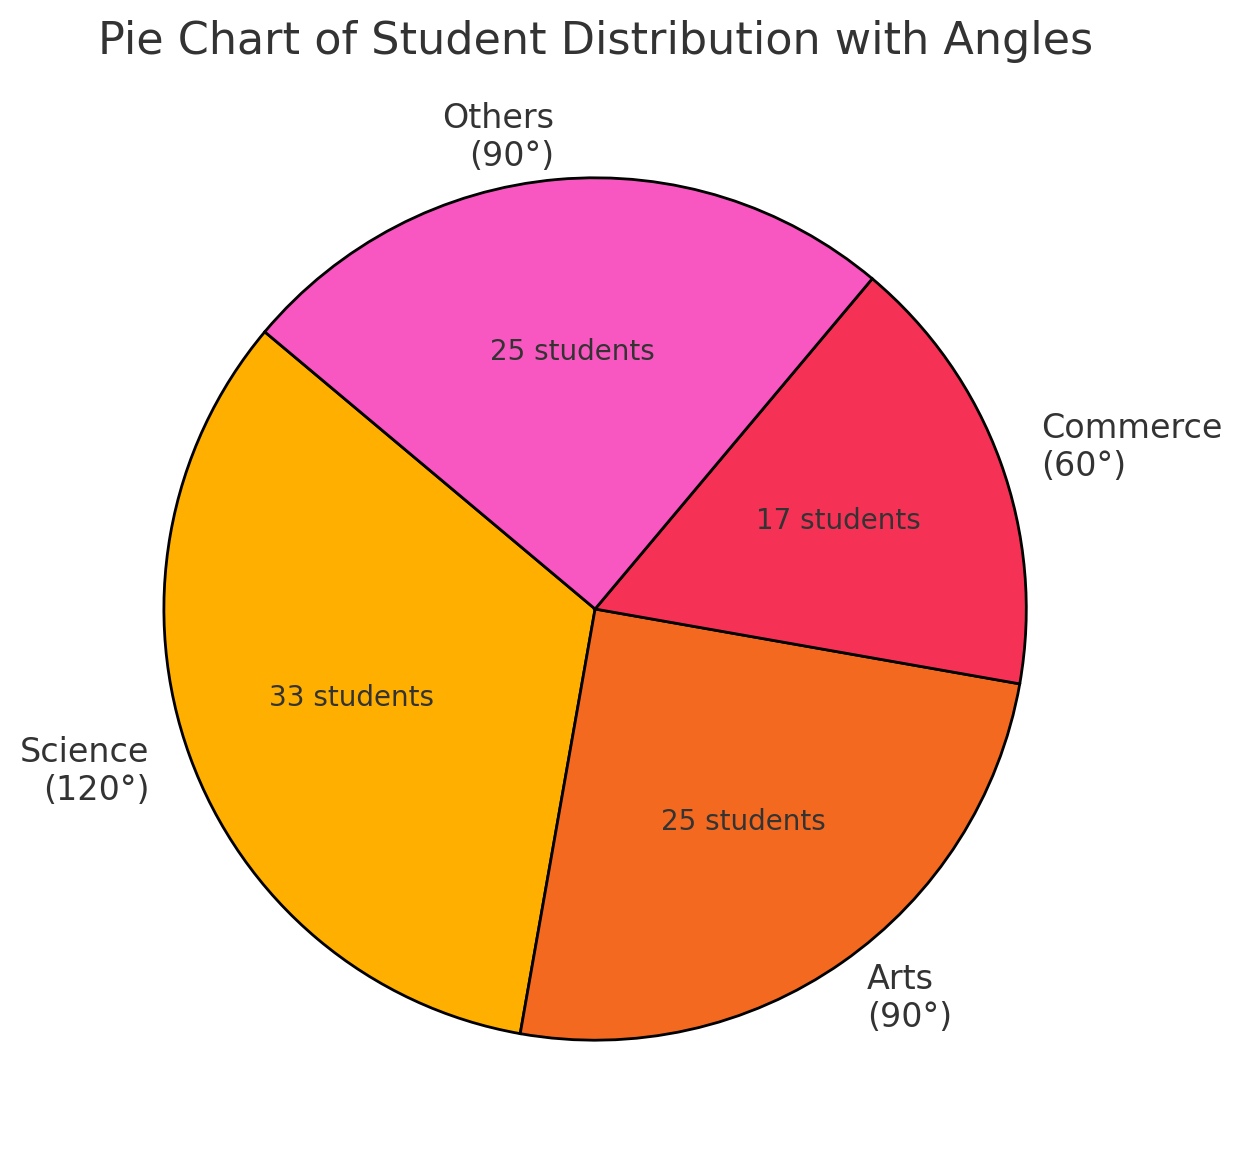
\includegraphics[width=0.6\textwidth]{5.2.png}
		\captionof{figure}{Pie chart representing student distribution.}
	\end{center}
	
	\vspace{0.5cm}
	\textbf{Solution:}
	\vspace{0.5cm}
	
	Let the angles of the pie chart sectors be:
	- Science: $120^\circ$
	- Arts: $90^\circ$
	- Commerce: $60^\circ$
	- Others: $90^\circ$
	
	The total angle in a pie chart is $360^\circ$, so we calculate each category as:
	\[
	\text{Number of students} = \frac{\text{sector angle}}{360^\circ} \times \text{total students}.
	\]
	
	\[
	\text{Science} = \frac{120}{360} \times 600 = 200.
	\]
	
	\[
	\text{Arts} = \frac{90}{360} \times 600 = 150.
	\]
	
	\[
	\text{Commerce} = \frac{60}{360} \times 600 = 100.
	\]
	
	\[
	\text{Others} = \frac{90}{360} \times 600 = 150.
	\]
	
	Thus, the number of students in each category is: Science = 200, Arts = 150, Commerce = 100, Others = 150.
\end{flushleft}

\begin{flushleft}
	\textbf{Example 5: Construct a cumulative frequency table and draw the cumulative frequency curve (ogive) for the following data.}
	
	\vspace{0.5cm}
	
	\begin{center}
		\begin{tabular}{c|c}
			\textbf{Class Interval} & \textbf{Frequency} \\
			\hline
			0-10 & 3 \\
			10-20 & 7 \\
			20-30 & 12 \\
			30-40 & 18 \\
			40-50 & 10 \\
		\end{tabular}
	\end{center}
	
	\vspace{0.5cm}
	\textbf{Solution:}
	\vspace{0.5cm}
	
	Step 1: Construct the cumulative frequency table by adding up the frequencies progressively.
	
	\vspace{0.5cm}
	
	\begin{center}
		\begin{tabular}{c|c|c}
			\textbf{Class Interval} & \textbf{Frequency} & \textbf{Cumulative Frequency} \\
			\hline
			0-10 & 3 & 3 \\
			10-20 & 7 & 3 + 7 = 10 \\
			20-30 & 12 & 10 + 12 = 22 \\
			30-40 & 18 & 22 + 18 = 40 \\
			40-50 & 10 & 40 + 10 = 50 \\
		\end{tabular}
	\end{center}
	
	\vspace{0.5cm}
	Step 2: Plot the cumulative frequency curve (ogive).
	
	\begin{center}
		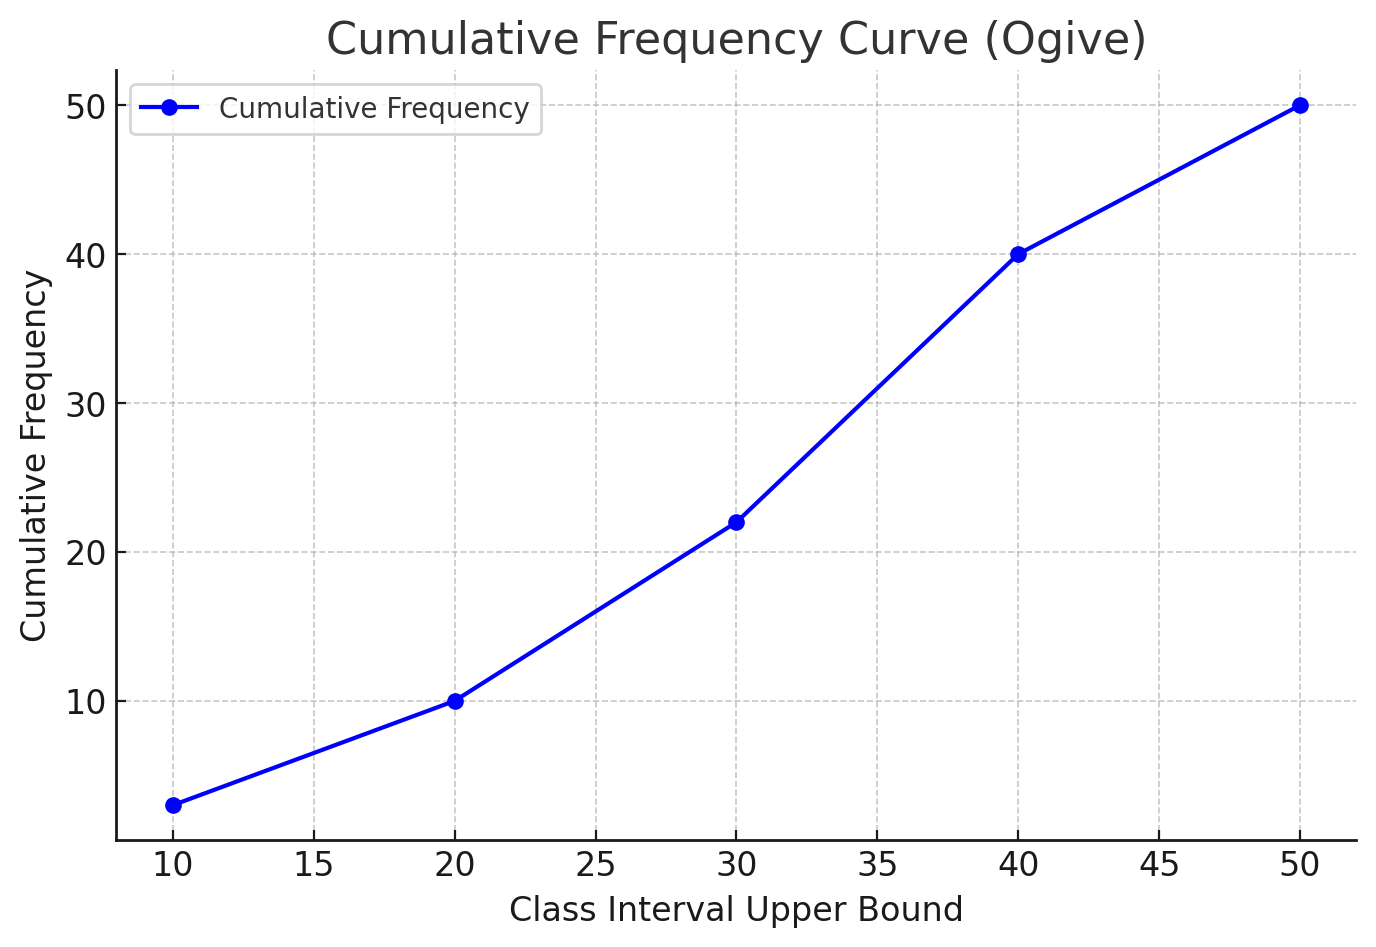
\includegraphics[width=0.6\textwidth]{5.3.png}
		\captionof{figure}{Cumulative Frequency Curve (Ogive)}
	\end{center}
	
	Step 3: Use the ogive to estimate the median and percentiles.
	
	- The median is the value corresponding to $\frac{n}{2} = \frac{50}{2} = 25$ on the cumulative frequency axis.
	- The 25th percentile is obtained at $\frac{50}{4} = 12.5$ on the cumulative frequency axis.
	- The 75th percentile is obtained at $\frac{3 \times 50}{4} = 37.5$ on the cumulative frequency axis.
	
	By tracing these values on the ogive, we estimate:
	\[
	\text{Median} \approx 27, \quad 25^\text{th} \text{ percentile} \approx 18, \quad 75^\text{th} \text{ percentile} \approx 35.
	\]
	
	Thus, the cumulative frequency curve helps in estimating key statistical measures.
\end{flushleft}
